\begin{comment}
All integrals in the weak forms in Eqs. \eqref{eq:PronghornEquations_V2WeakForm}-\eqref{eq:MultiscaleWeak} are written in terms of the ``physical'' coordinates, or the \(x_1\), \(x_2\), and \(x_3\) coordinates defining the domain. Each physical element is stretched and compressed through a coordinate transformation to an element in the ``master'' coordinates, or the \(\xi_1\), \(\xi_2\), and \(\xi_3\) coordinates defining a reference element. Fig. \ref{fig:physical} shows a schematic of the physical element highlighted in Fig. \ref{fig:fe_mesh} and Fig. \ref{fig:master} shows the same element when transformed to the master domain.

\begin{figure}[!h]
\centering
\begin{subfigure}{.485\textwidth}
  \centering
  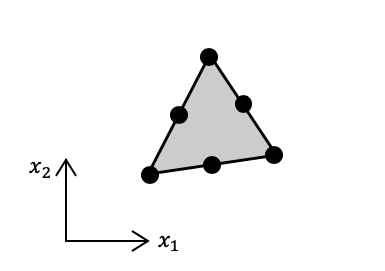
\includegraphics[width=0.8\linewidth]{figs/physical_elem.png}
  \caption{Physical element}
  \label{fig:physical}
\end{subfigure}
\begin{subfigure}{.485\textwidth}
  \centering
  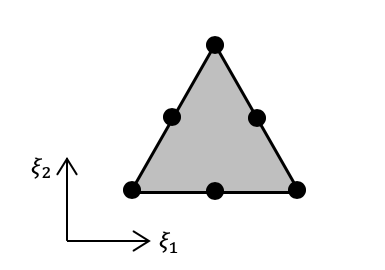
\includegraphics[width=0.8\linewidth]{figs/master_elem.png}
  \caption{Master element}
  \label{fig:master}
\end{subfigure}
\caption{Schematic of a (a) physical element and (b) the master element.}
\label{fig:physical_master}
\end{figure}

Transformation between the two domains is given as

\beq
\label{eq:JacobianMasterPhysical}
dx_i=\frac{\partial x_i}{\partial \xi_j}d\xi_j\ ,
\eeq

\noindent where an isoparametric mapping in terms of the physical node coordinates \(X_i\) and master domain basis functions is used,

\beq
x_i(\vec{\xi})=\sum_{i\ =\ 1}^{n_{en}}X_i\phi_i(\vec{\xi})\ .
\eeq

\noindent Mappings of boundary integrals are described elsewhere \cite{zohdi}. The mapping between physical and master domains enables all integrals in the weak form to use the same quadrature rule, shape functions, and weight functions. 
\end{comment}

